%Version 3 October 2023
% See section 11 of the User Manual for version history
%
%%%%%%%%%%%%%%%%%%%%%%%%%%%%%%%%%%%%%%%%%%%%%%%%%%%%%%%%%%%%%%%%%%%%%%
%%                                                                 %%
%% Please do not use \input{...} to include other tex files.       %%
%% Submit your LaTeX manuscript as one .tex document.              %%
%%                                                                 %%
%% All additional figures and files should be attached             %%
%% separately and not embedded in the \TeX\ document itself.       %%
%%                                                                 %%
%%%%%%%%%%%%%%%%%%%%%%%%%%%%%%%%%%%%%%%%%%%%%%%%%%%%%%%%%%%%%%%%%%%%%

%%\documentclass[referee,sn-basic]{sn-jnl}% referee option is meant for double line spacing

%%=======================================================%%
%% to print line numbers in the margin use lineno option %%
%%=======================================================%%

%%\documentclass[lineno,sn-basic]{sn-jnl}% Basic Springer Nature Reference Style/Chemistry Reference Style

%%======================================================%%
%% to compile with pdflatex/xelatex use pdflatex option %%
%%======================================================%%

%%\documentclass[pdflatex,sn-basic]{sn-jnl}% Basic Springer Nature Reference Style/Chemistry Reference Style


%%Note: the following reference styles support Namedate and Numbered referencing. By default the style follows the most common style. To switch between the options you can add or remove �Numbered� in the optional parenthesis. 
%%The option is available for: sn-basic.bst, sn-vancouver.bst, sn-chicago.bst%  
 
\documentclass[sn-nature]{sn-jnl}% Style for submissions to Nature Portfolio journals
%%\documentclass[sn-basic]{sn-jnl}% Basic Springer Nature Reference Style/Chemistry Reference Style
%%\documentclass[sn-mathphys-num]{sn-jnl}% Math and Physical Sciences Numbered Reference Style 
%%\documentclass[sn-mathphys-ay]{sn-jnl}% Math and Physical Sciences Author Year Reference Style
%%\documentclass[sn-aps]{sn-jnl}% American Physical Society (APS) Reference Style
%%\documentclass[sn-vancouver,Numbered]{sn-jnl}% Vancouver Reference Style
%%\documentclass[sn-apa]{sn-jnl}% APA Reference Style 
%%\documentclass[sn-chicago]{sn-jnl}% Chicago-based Humanities Reference Style

%%%% Standard Packages
%%<additional latex packages if required can be included here>

\usepackage{graphicx}%
\usepackage{multirow}%
\usepackage{amsmath,amssymb,amsfonts}%
\usepackage{amsthm}%
\usepackage{mathrsfs}%
\usepackage[title]{appendix}%
\usepackage{xcolor}%
\usepackage{textcomp}%
\usepackage{manyfoot}%
\usepackage{booktabs}%
\usepackage{algorithm}%
\usepackage{algorithmicx}%
\usepackage{algpseudocode}%
\usepackage{listings}%
\usepackage[justification=centering]{caption}%
%%%%

%%%%%=============================================================================%%%%
%%%%  Remarks: This template is provided to aid authors with the preparation
%%%%  of original research articles intended for submission to journals published 
%%%%  by Springer Nature. The guidance has been prepared in partnership with 
%%%%  production teams to conform to Springer Nature technical requirements. 
%%%%  Editorial and presentation requirements differ among journal portfolios and 
%%%%  research disciplines. You may find sections in this template are irrelevant 
%%%%  to your work and are empowered to omit any such section if allowed by the 
%%%%  journal you intend to submit to. The submission guidelines and policies 
%%%%  of the journal take precedence. A detailed User Manual is available in the 
%%%%  template package for technical guidance.
%%%%%=============================================================================%%%%

%% as per the requirement new theorem styles can be included as shown below
\theoremstyle{thmstyleone}%
\newtheorem{theorem}{Theorem}%  meant for continuous numbers
%%\newtheorem{theorem}{Theorem}[section]% meant for sectionwise numbers
%% optional argument [theorem] produces theorem numbering sequence instead of independent numbers for Proposition
\newtheorem{proposition}[theorem]{Proposition}% 
%%\newtheorem{proposition}{Proposition}% to get separate numbers for theorem and proposition etc.

\theoremstyle{thmstyletwo}%
\newtheorem{example}{Example}%
\newtheorem{remark}{Remark}%

\theoremstyle{thmstylethree}%
\newtheorem{definition}{Definition}%

\raggedbottom
%%\unnumbered% uncomment this for unnumbered level heads

\begin{document}

\title[Pistachio Supply Chain Optimization]{Pistachio Supply Chain Optimization}

%%=============================================================%%
%% GivenName	-> \fnm{Joergen W.}
%% Particle	-> \spfx{van der} -> surname prefix
%% FamilyName	-> \sur{Ploeg}
%% Suffix	-> \sfx{IV}
%% \author*[1,2]{\fnm{Joergen W.} \spfx{van der} \sur{Ploeg} 
%%  \sfx{IV}}\email{iauthor@gmail.com}
%%=============================================================%%

\author[1]{\fnm{Raissa} \sur{Gonçalves Diniz}}\email{raissagd@ufmg.br}

\author[1,2]{\fnm{André} \sur{Costa Batista}}\email{andre-costa@ufmg.br}

\affil[1]{\orgdiv{Operations Research and Complex Systems Laboratory}, \orgname{Universidade Federal de Minas Gerais}, \orgaddress{\country{Brazil}}}

\affil[2]{\orgdiv{Department of Electrical Engineering}, \orgname{Universidade Federal de Minas Gerais}, \orgaddress{\street{Av. Antônio Carlos 6627}, \city{Belo Horizonte}, \postcode{31270-010}, \state{Minas Gerais}, \country{Brazil}}}


%%==================================%%
%% Sample for unstructured abstract %%
%%==================================%%

\abstract{The abstract serves both as a general introduction to the topic and as a brief, non-technical summary of the main results and their implications. Authors are advised to check the author instructions for the journal they are submitting to for word limits and if structural elements like subheadings, citations, or equations are permitted.}

%%================================%%
%% Sample for structured abstract %%
%%================================%%

% \abstract{\textbf{Purpose:} The abstract serves both as a general introduction to the topic and as a brief, non-technical summary of the main results and their implications. The abstract must not include subheadings (unless expressly permitted in the journal's Instructions to Authors), equations or citations. As a guide the abstract should not exceed 200 words. Most journals do not set a hard limit however authors are advised to check the author instructions for the journal they are submitting to.
% 
% \textbf{Methods:} The abstract serves both as a general introduction to the topic and as a brief, non-technical summary of the main results and their implications. The abstract must not include subheadings (unless expressly permitted in the journal's Instructions to Authors), equations or citations. As a guide the abstract should not exceed 200 words. Most journals do not set a hard limit however authors are advised to check the author instructions for the journal they are submitting to.
% 
% \textbf{Results:} The abstract serves both as a general introduction to the topic and as a brief, non-technical summary of the main results and their implications. The abstract must not include subheadings (unless expressly permitted in the journal's Instructions to Authors), equations or citations. As a guide the abstract should not exceed 200 words. Most journals do not set a hard limit however authors are advised to check the author instructions for the journal they are submitting to.
% 
% \textbf{Conclusion:} The abstract serves both as a general introduction to the topic and as a brief, non-technical summary of the main results and their implications. The abstract must not include subheadings (unless expressly permitted in the journal's Instructions to Authors), equations or citations. As a guide the abstract should not exceed 200 words. Most journals do not set a hard limit however authors are advised to check the author instructions for the journal they are submitting to.}

\keywords{keyword1, Keyword2, Keyword3, Keyword4}

%%\pacs[JEL Classification]{D8, H51}

%%\pacs[MSC Classification]{35A01, 65L10, 65L12, 65L20, 65L70}

\maketitle

\section{Introduction}\label{sec1}

Lorem ipsum dolor sit amet, consectetur adipiscing elit. Sed cursus ullamcorper ante vel tempor. 
Curabitur tincidunt leo ligula, at faucibus sem porttitor non. Proin sodales, ex malesuada dictum cursus, 
libero massa feugiat erat, convallis sollicitudin ante arcu non ante. Curabitur vitae neque pretium, 
placerat quam quis, porttitor metus. In suscipit orci at lectus sollicitudin, vel porta sem tempor. 
Integer posuere, libero non eleifend imperdiet, nisl elit ultrices dolor, auctor fringilla libero 
justo eget leo. Curabitur maximus libero pharetra felis porta, quis elementum massa fermentum. 

\section{Problem definition}

The proposed network includes producers, processing centers, pistachio factories, 
oil extraction centers, composting centers, and customers. Pistachios are transported 
from orchards to processing centers, producing open-mouth pistachios, raw kernels, and 
waste, which are then sent to factories, oil extraction centers, and composting centers, respectively. 
Open-mouth pistachios are roasted, packed, and shipped to customers, while pistachio oil 
is delivered to oil customers and cosmetic factories. Waste is converted into compost for 
distribution. The model aims to minimize total costs \eqref{eq:custo}, including opening, transportation,
and production costs, under the following capacity and demand constraints with no allowed shortages:
    
\begin{align}
    \min &\ z_1 + z_2 + z_3 \label{eq:custo}\\
    \text{s.t.} \quad & \sum\limits_{j=1}^J X_{ij} \le Cpa_i, \quad \forall i \in I \label{eq:restricao1}\\
    & \sum\limits_{i=1}^I X_{ij} \le Cpu_j\times U_j, \quad \forall j \in J \label{eq:restricao2}\\
    & \sum\limits_{e=1}^E Ow_{eq} + \sum\limits_{j=1}^J Gw_{jq} \le Cpy_q \times T_q, \quad \forall q \in Q \label{eq:restricao3}\\
    & \sum\limits_{j=1}^J Go_{jk} \le Cpw_k\times W_k, \quad \forall k \in K \label{eq:restricao4}\\
    & \sum\limits_{j=1}^J Gr_{je} \le Cpr_e\times R_e, \quad \forall e \in E \label{eq:restricao5}\\
    & \sum\limits_{e=1}^E O_{en_2} \le Cpv_s\times V_s, \quad \forall s \in S \label{eq:restricao6}\\
    & \sum\limits_{k=1}^K Go_{jk} + \sum\limits_{e=1} Gr_{je} + \sum\limits_{q=1}^Q Gw_{jq} \le \sum\limits_{i=1} X_{ij}, \quad \forall j \in J \label{eq:restricao7} \\
    & \sum\limits_{k=1}^K Go_{jk} = (1-\beta) \sum\limits_{i=1}^I X_{ij}\theta_1, \quad \forall j\in J \label{eq:restricao8}\\
    & \sum\limits_{e=1}^K Gr_{je} = (1-\beta) \sum\limits_{i=1}^I X_{ij}\theta_2, \quad \forall j\in J \label{eq:restricao9}\\
    & \sum\limits_{q=1}^Q Gw_{jq} = \sum\limits_{i=1}^I X_{ij}\theta_3, \quad \forall j\in J \label{eq:restricao10}\\
    & \theta_1 + \theta_2 + \theta_3 = 1 \label{eq:restricao11}\\
    & \sum\limits_{n_1=1}^{N_1} P_{kn_1} \le \sum\limits_{j=1}^J Go_{jk} \times \gamma k, \quad \forall k \in K \label{eq:restricao12}\\
    & \sum\limits_{n_2=1}^{N_2} O_{en_2} + \sum\limits_{s=1}^S Oc_{es} \le \sum\limits_{j=1} Gr_{je}\times(1-\lambda), \quad \forall e\in E \label{eq:restricao13}\\
    & \sum\limits_{q=1}^{Q} Ow_{eq} \le \sum\limits_{j=1}^J Gr_{je} \times \lambda k, \quad \forall e \in E \label{eq:restricao14}\\
    & \sum\limits_{n_3=1}^{N_3} L_{sn_1} \le \sum\limits_{e=1}^E Oc_{es} \times \gamma s, \quad \forall s \in S \label{eq:restricao15}\\
    & \sum\limits_{m=1}^M D_{qm} \le \left(\sum\limits_{j=1}^J Gw_{jq} + \sum\limits_{e=1}^E Ow_{eq} \right) \times \gamma q, \quad \forall q \in Q \label{eq:restricao16}\\
    & \sum\limits_{k=1}^K P_{kn_1} \le Dp_{n_1}, \quad \forall n_1 \in N_1 \label{eq:restricao17}\\
    & \sum\limits_{e=1}^E O_{en_2} \le Du_{n_2}, \quad \forall n_2 \in N_2 \label{eq:restricao18}\\
    & \sum\limits_{s=1}^S L_{sn_3} \le Ds_{n_3}, \quad \forall n_3 \in N_3 \label{eq:restricao19}\\
    & \sum\limits_{q=1}^Q D_{qm} \le Dc_{m}, \quad \forall m \in M \label{eq:restricao20}
\end{align}

    
\begin{itemize}
    \item The objective function \eqref{eq:custo} minimizes the total costs of the supply chain, including opening, transportation, and production costs. The costs are divided into three components: 
    $z_1$ \eqref{eq:custo1}, $z_2$ \eqref{eq:custo2}, and $z_3$ \eqref{eq:custo3}, which represent the costs of opening facilities, transportation, and production, respectively as shown in the following equations:
    \begin{align}
        z_1 &= \sum\limits_{j=1}^J Fu_j\times U_j 
        + \sum\limits_{q=1}^Q Fy_q\times Y_q
        + \sum\limits_{k=1}^{K} Fw_k\times W_k
        + \sum\limits_{e=1}^{E} Fr_e\times R_e
        + \sum\limits_{s=1}^S Fv_s\times V_s \label{eq:custo1}\\
        z_2 &= \sum\limits_{i=1}^I\sum\limits_{j=1}^J CI_i\times X_{ij} 
        + \sum\limits_{j=1}^J\sum\limits_{k=1}^K Cu_{1j}\times Go_{jk}
        + \sum\limits_{j=1}^J\sum\limits_{e=1}^E Cu_{2j}\times Gr_{je} \nonumber \\
        &+ \sum\limits_{q=1}^Q\sum\limits_{m=1}^M Cy_{q}\times D_{qm} 
        + \sum\limits_{k=1}^K\sum\limits_{n_1=1}^{N_1} Cw_{k}\times P_{kn_1} \nonumber \\
        &+ \sum\limits_{e=1}^E Cr_e\left(\sum\limits_{n_2=1}^{N_2}O_{en_2} 
        + \sum\limits_{s=1}^S Oc_{es}\right)
        + \sum\limits_{s=1}^S\sum\limits_{n_3=1}^{N_3} Cv_{s}\times L_{sn_3} \label{eq:custo2}\\ 
        z_3 &= \sum\limits_{i=1}^I\sum\limits_{j=1}^J CX_{ij}\times X_{ij} 
        + \sum\limits_{j=1}^J\sum\limits_{k=1}^K CK_{jk}\times Go_{jk}
        + \sum\limits_{j=1}^J\sum\limits_{q=1}^Q CJ_{jq}\times Gw_{jq} \nonumber \\
        &+ \sum\limits_{e=1}^E\sum\limits_{s=1}^S CS_{es}\times Oc_{es} 
        + \sum\limits_{e=1}^E\sum\limits_{n_2=1}^{N_2} CN_{en_2}\times Oc_{en_2}
        + \sum\limits_{e=1}^E\sum\limits_{q=1}^Q CQ_{eq}\times Ow_{eq} \nonumber \\
        &+ \sum\limits_{s=1}^S\sum\limits_{n_3=1}^{N_3} Cl_{sn_3}\times L_{sn_3} 
        + \sum\limits_{k=1}^K\sum\limits_{n_1=1}^{N_1} Cp_{kn_1}\times P_{kn_1} 
        + \sum\limits_{q=1}^Q\sum\limits_{m=1}^M Cd_{qm}\times D_{qm} \label{eq:custo3}
    \end{align}
    \item The variables $R_j$, $Y_q$, $W_k$, $Z_e$, and $V_s$ are binary decision variables that indicate whether certain elements in the model are active. 
    For example, $R_j = 1$ if facility $j$ is open, and 0 otherwise. The other variables in the model are continuous and positive, representing real numbers 
    greater than or equal to zero, used for modeling flows, quantities, and other measurable factors.
    \item The constraints \eqref{eq:restricao1}-\eqref{eq:restricao6} address the finite capacities and demands of each center within the supply chain. Specifically, constraint \eqref{eq:restricao1} limits the quantity of 
    products shipped from producers to distribution centers. Constraints \eqref{eq:restricao2}-\eqref{eq:restricao6} then ensure that the quantities of products delivered to processing centers, compost 
    centers, pistachio factories, oil extraction centers, and cosmetic factories do not exceed the capacities of these centers.
    \item Products sent from any center must not exceed the orders received by that center. Therefore, constraint \eqref{eq:restricao7} stipulates that the quantity of products 
    shipped from a processing center must be less than or equal to the quantity delivered to other centers. 
    Constraints \eqref{eq:restricao8}-\eqref{eq:restricao11} specify the quantities of open-mouth pistachios, raw kernels, and waste produced through the dehulling process at each processing center. 
    Similarly, constraints \eqref{eq:restricao12}-\eqref{eq:restricao16} regulate the flows within pistachio factories, oil extraction centers, cosmetic factories, and composting centers. 
    \item Finally, to ensure that customer demand is met, constraints \eqref{eq:restricao17}-\eqref{eq:restricao20} guarantee that the products delivered to pistachio customers, pistachio oil customers, 
    cosmetic customers, and compost markets meet or exceed their respective demands.
\end{itemize}
    
\section{Heuristic approach}

In this section, we present the methodology employed to address the optimization problem. The proposed approach 
integrates priority-based encoding and the Variable Neighborhood Search (VNS) algorithm, 
which together form the core of our solution strategy. We begin by detailing the solution representation, 
which utilizes priority-based encoding to efficiently manage and rank decision variables, allowing for effective 
exploration of the solution space. This encoding scheme is crucial in guiding the search process and maintaining 
feasibility while optimizing the objective function. Following this, we delve into the VNS algorithm, a robust 
metaheuristic known for its flexibility and capacity to escape local optima through systematic changes in 
neighborhood structures. The algorithm dynamically adjusts between multiple neighborhood structures, each 
designed to explore different aspects of the solution landscape, thereby enhancing the search process. 
We will also discuss the specific configurations and parameters used, as well as the design of neighborhood 
operators tailored to the problem characteristics. This comprehensive approach aims to deliver a high-quality 
solution by leveraging the strengths of priority-based encoding and the adaptability of VNS.

\subsection{Solution representation}
In this work, a priority-based encoding scheme is used to represent the solution space effectively, drawing on chromosome-based 
representations where each gene corresponds to a node (source or depot) in the transportation problem \cite{gen2006genetic}. 
The transportation problem is modeled as a tree structure, with nodes representing sources or depots and edges representing 
transportation arcs. The primary objective is to construct a transportation tree that meets all depot demands while minimizing 
total transportation costs.

Each chromosome encodes the priority of nodes, guiding the construction of the transportation tree by establishing the most 
cost-effective connections first. The decoding process starts by identifying the node with the highest priority in the chromosome 
and connecting it to the corresponding node with the lowest transportation cost. For instance, if Depot 1 has the highest priority, 
it is linked to the source that offers the lowest cost connection to Depot 1. The shipment amount is determined by the minimum of 
the source's capacity and the depot's demand. Once the shipment is fulfilled, the depot's priority is updated (or set to zero if 
its demand is satisfied), and the process continues with the next highest priority node. This sequential process of arc appending 
and priority updating repeats until all depots' demands are satisfied, resulting in a complete transportation tree.

The supply chain is determined using a step-by-step, backward approach, starting from consumer demand and moving upward toward producers. 
This method ensures resource allocation is optimized at each stage, preventing excess or unnecessary material flow. For example, 
after determining the quantity of open-mouth pistachios required by consumers, we work backward to calculate the factories' 
processing needs, ensuring their capacities are not overloaded. This then informs how much material the processing centers must supply, 
aligning each upstream stage with the final demand and optimizing resource use throughout the chain.

\begin{figure}[h!]
    \centering
    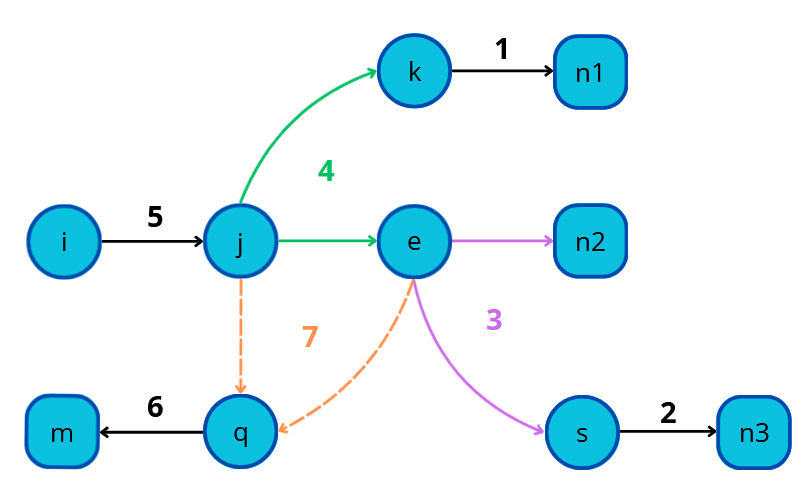
\includegraphics[width=0.8\textwidth]{./imgs/decode_flux.PNG}
    \caption{Decodification steps of the transportation tree}
    \label{fig:decode_flux}
\end{figure}

As shown in Figure~\ref{fig:decode_flux}, the decoding process begins with the flow of pistachio products from factories to consumers, ensuring that 
all constraints are met: consumer demand is satisfied, the total amount of product leaving the factory does not exceed the 
pistachio received from processing centers multiplied by the factory’s production rate, and the pistachio sent to any active 
factory is within its capacity. Likewise, the distribution of cosmetic products from factories to consumers and the transfer of oil 
from extraction centers to both oil consumers and cosmetic factories adhere to the same principles, ensuring all constraints are satisfied

The flow from processing centers to pistachio factories and oil extraction centers is regulated by constraints ensuring that the 
total pistachios leaving a processing center do not exceed the harvested amount sent by producers. Harvested pistachios are divided into three parts, 
each assigned to a product type, with a $(1-\beta)$ loss factor applied to pistachios with shells and pits. Factories can receive more pistachios than 
they process, but must meet a minimum intake, while oil extraction centers send no more than $(1-\lambda)$ of the kernels to consumers and cosmetics factories, 
with the remaining $\lambda$ going to composting. All processing centers must respect their capacity limits to ensure efficient distribution.

The decoding process for this specific flow is more complex and requires a targeted approach. First, we must determine the flow of in-shell pistachios from 
processing centers to pistachio factories, and the flow of kernels from processing centers to oil extraction centers. Using the given constraints, we calculate 
the quantity of harvested pistachios each processing center must receive to meet the demands of both pistachio factories and oil extraction centers.

If the factory demand exceeds that of the oil extraction centers, the processing center must prioritize meeting the exact demand of the factories. Since 
harvested pistachios are divided into three proportional parts, basing the allocation solely on the oil extraction center’s demand would leave the factories 
undersupplied. The priority should be given to the entity with the greatest need, adjusting the remaining flow accordingly, as constraints allow for over-supply 
but not shortages.

Thus, we need to adjust the quantity of kernels shipped from the processing centers to the oil extraction centers, ensuring enough is sent to satisfy the 
restrictions. This involves calculating the total amount of kernels required, identifying the oil extraction center with the lowest transportation cost, and 
directing the additional flow there to minimize costs.

If, instead, the oil extraction centers have higher demand, the process is reversed: the pistachio factories' flow is adjusted accordingly to balance 
the supply while minimizing transportation costs.

Next, the flow of harvested pistachios from producers to processing centers is also governed by constraints ensuring that no producer exceeds its production 
capacity and no processing center receives more than it can process. While the capacity of each producer limits the supply, the demand for each 
processing center has already been determined in a previous step. If producers' capacities are insufficient to meet the total demand, the solution 
becomes infeasible. However, due to the constraints on product allocation between processing centers, this flow will always satisfy the condition of equality.

Similarly, the flow of fertilizer from composting centers to consumers is governed by constraints that ensure composting centers do not receive more waste than 
they can handle. The amount of fertilizer sent must be less than or equal to the waste received from processing and oil extraction centers, adjusted by the 
composting center's production rate. Finally, for the waste flow from processing and oil extraction centers to composting centers, constraints also ensure that no 
composting center receives more waste than its capacity. Waste from each processing center is assigned to the composting center with the lowest associated cost, 
ensuring that no composting center receives more waste than required. If the waste sent to a composting center falls short of its needs, the demand is adjusted 
accordingly. Conversely, if excess waste is sent, the demand is set to zero. Once all processing centers have allocated their waste, any remaining composting 
needs are fulfilled by oil extraction centers, considering their available capacity. If no additional waste is needed, no waste is sent from the oil extraction 
centers. Finally, the total cost of transporting waste is updated based on the assignments, ensuring efficient waste management across the supply chain.


\subsection{VNS algorithm}
The Variable Neighborhood Search (VNS) algorithm is a powerful metaheuristic that combines local search with
systematic changes in neighborhood structures to explore the solution space effectively. By iteratively
applying different neighborhood operators, VNS can escape local optima and discover high-quality solutions
through continuous diversification and intensification phases. 

The algorithm begins by initializing a solution and setting the maximum neighborhood size and time limit. 
It then enters a loop, where it repeatedly applies the shaking and local search procedures to generate new candidate solutions. 
If a better solution is found, it replaces the current best solution and resets the neighborhood size. 
Otherwise, the algorithm increases the neighborhood size and continues the search. The process repeats until the time limit 
is reached, at which point the best found solution is returned. Algorithm~\ref{algoVNS} provides a detailed outline of 
the VNS algorithm.

\begin{algorithm}
    \caption{Variable Neighborhood Search (VNS)}\label{algoVNS}
    \begin{algorithmic}[1]
    \Require Initial solution $x$, maximum neighborhood size $k_{\text{max}}$, time limit $t_{\text{max}}$
    \Ensure Best found solution $x^*$
    \State $x^* \Leftarrow x$
    \Repeat
        \State $k \Leftarrow 1$
        \Repeat
            \State $x' \Leftarrow \text{Shake}(x, k)$ \Comment{Shaking}
            \State $x'' \Leftarrow \text{LocalSearch}(x')$ \Comment{Local search}
            \If{$f(x'') < f(x^*)$}
                \State $x^* \Leftarrow x''$
                \State $k \Leftarrow 1$ \Comment{Reset neighborhood size}
            \Else
                \State $k \Leftarrow k + 1$
            \EndIf
        \Until{$k > k_{\text{max}}$}
        \State $t \Leftarrow \text{CpuTime}()$
    \Until{$t > t_{\text{max}}$}
    \end{algorithmic}
\end{algorithm}

\subsection{Neighborhood structures}
In the context of the Variable Neighborhood Search (VNS) algorithm, neighborhood operators play a crucial role 
in exploring the solution space by systematically altering the current solution to generate new candidate solutions. 
The effectiveness of VNS relies heavily on the design and application of these operators, as they determine the 
diversity and direction of the search process. In this study, we utilize four classic neighborhood operators: 
Swap, Reversion, Insertion, and Slide. Each operator perturbs the solution in a distinct manner, allowing the 
algorithm to escape local optima and explore different regions of the search space. By iteratively applying 
these operators, VNS enhances its capability to find high-quality solutions through continuous diversification 
and intensification phases. The neighborhood structures used are detailed below, and illustraed in Figure~\ref{fig:nbdh_op}.:

\begin{itemize}
    \item \textbf{Swap:} The swap operator exchanges the positions of two selected elements within the chromosome. 
    In the example, the selected elements are 6 and 3. This operator is useful for making quick adjustments to 
    the order of elements without altering the overall structure significantly.
    \item \textbf{Reversion:} The reversion operator reverses the order of all elements between the two selected indices. In this case, with elements 6 and 3 chosen, 
    the operator reverses the sequence between these two points. This operation can effectively rearrange subsequences, potentially moving the solution 
    closer to a local optimum by drastically altering a segment of the sequence.
    \item \textbf{Insertion:} In this operation, the unit in the second selected position is relocated immediately after the unit in the first position. 
    Subsequently, all units that were originally between these positions are shifted accordingly to the right. This allows the algorithm to make focused 
    adjustments by repositioning a specific element within the sequence while maintaining the overall order of the other elements.
    \item \textbf{Slide:} This operator begins by selecting two units of a solution randomly, like the other three. The first unit is removed, and the units 
    that were initially located between the two selected units are shifted toward the start position of the first unit. Finally, the initially 
    removed unit is placed at the position of the second unit. This sliding mechanism creates a subtle yet impactful reordering of the solution elements, 
    which can enhance the search process by generating new configurations with minimal disruption.
\end{itemize}

\begin{figure}[h!]
    \centering
    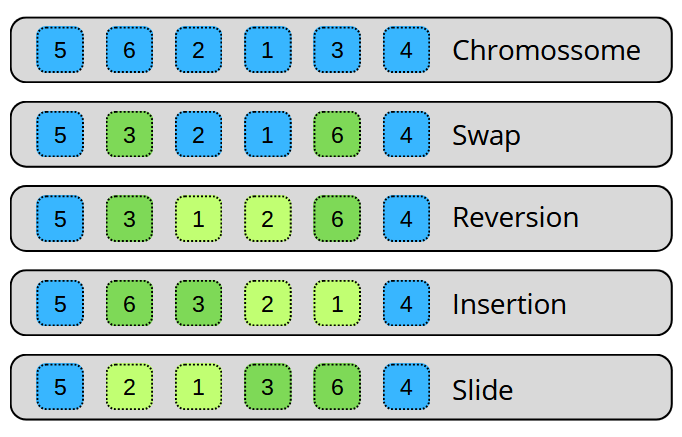
\includegraphics[width=0.8\textwidth]{./imgs/nbhd_op.png}
    \caption{Neighborhood structures used in the VNS Algorithm}
    \label{fig:nbdh_op}
\end{figure}

\section{Results}
    
Lorem ipsum dolor sit amet, consectetur adipiscing elit. Sed cursus ullamcorper ante vel tempor. 
Curabitur tincidunt leo ligula, at faucibus sem porttitor non. Proin sodales, ex malesuada dictum cursus, 
libero massa feugiat erat, convallis sollicitudin ante arcu non ante. Curabitur vitae neque pretium, 
placerat quam quis, porttitor metus. In suscipit orci at lectus sollicitudin, vel porta sem tempor. 
Integer posuere, libero non eleifend imperdiet, nisl elit ultrices dolor, auctor fringilla libero 
justo eget leo. Curabitur maximus libero pharetra felis porta, quis elementum massa fermentum.    
    
\begin{table}[h]
    \caption{Average solution values and execution times of the VNS algorithm compared to the Exact Algorithm (Gurobi).}\label{tab2}
    \begin{tabular*}{\textwidth}{@{\extracolsep\fill}lcccccc}
    \toprule%
    & \multicolumn{3}{@{}c@{}}{Solution value} & \multicolumn{3}{@{}c@{}}{Execution time} \\\cmidrule{2-4}\cmidrule{5-7}%
    Instance & VNS & Gurobi & Difference & VNS & Gurobi & Difference \\
    \midrule
    100 & 7.356017e+06 & 7059878.15 & 4.19\% & 240.576739s & 261s & -7.83\%\\
    200 & 1.488441e+08 & 137535570.42 &  8.22\%  & 714.499149s & 3834s & -81.36\%\\
    400 & 3.075344e+08 & 270662192.84 & 13.62\%  & 2015.728858s & 70339s & -97.13\%\\
    800 & 6.573093e+08 & 547200537.38 & 20.12\%  & 5537.291645s & 11836s&  -53.22\%\\
    1600 & 1.364413e+09 & - & - & 17766.873715s & - & -\\
    \botrule
    \end{tabular*}
\end{table}

\begin{table}[h]
    \caption{Average solution values of the VNS algorithm compared to the Genetic Algorithm (GA).}\label{tab2}
    \begin{tabular*}{\textwidth}{@{\extracolsep\fill}lcccccc}
    \toprule%
    & \multicolumn{3}{@{}c@{}}{Solution value}\\\cmidrule{2-4}\cmidrule{5-7}%
    Instance & VNS & GA & Difference\\
    \midrule
    100 & 74105277.59 & 74630611.96 & 0.71\%\\
    200 & 150165899.77 & 155311143.01 &  3.37\%\\
    400 & 307527336.72 & 324315714.06  & 5.31\%\\
    800 & 657000372.14 & 692477371.5  & 5.26\%\\
    1600& 1363240244.41 & -  & -\\
    \botrule
    \end{tabular*}
\end{table}


\section{Conclusion}

Lorem ipsum dolor sit amet, consectetur adipiscing elit. Sed cursus ullamcorper ante vel tempor. 
Curabitur tincidunt leo ligula, at faucibus sem porttitor non. Proin sodales, ex malesuada dictum cursus, 
libero massa feugiat erat, convallis sollicitudin ante arcu non ante. Curabitur vitae neque pretium, 
placerat quam quis, porttitor metus. In suscipit orci at lectus sollicitudin, vel porta sem tempor. 
Integer posuere, libero non eleifend imperdiet, nisl elit ultrices dolor, auctor fringilla libero 
justo eget leo. Curabitur maximus libero pharetra felis porta, quis elementum massa fermentum. 

\section{Cross referencing}\label{sec8}

Environments such as figure, table, equation and align can have a label
declared via the \verb+\label{#label}+ command. For figures and table
environments use the \verb+\label{}+ command inside or just
below the \verb+\caption{}+ command. You can then use the
\verb+\ref{#label}+ command to cross-reference them. As an example, consider
the label declared for Figure~\ref{fig1} which is
\verb+\label{fig1}+. To cross-reference it, use the command 
\verb+Figure \ref{fig1}+, for which it comes up as
``Figure~\ref{fig1}''. 

To reference line numbers in an algorithm, consider the label declared for the line number 2 of Algorithm~\ref{algo1} is \verb+\label{algln2}+. To cross-reference it, use the command \verb+\ref{algln2}+ for which it comes up as line~\ref{algln2} of Algorithm~\ref{algo1}.

\subsection{Details on reference citations}\label{subsec7}

Standard \LaTeX\ permits only numerical citations. To support both numerical and author-year citations this template uses \verb+natbib+ \LaTeX\ package. For style guidance please refer to the template user manual.

Here is an example for \verb+\cite{...}+: \cite{bib1}. Another example for \verb+\citep{...}+: \citep{bib2}. For author-year citation mode, \verb+\cite{...}+ prints Jones et al. (1990) and \verb+\citep{...}+ prints (Jones et al., 1990).

All cited bib entries are printed at the end of this article: \cite{bib3}, \cite{bib4}, \cite{bib5}, \cite{bib6}, \cite{bib7}, \cite{bib8}, \cite{bib9}, \cite{bib10}, \cite{bib11}, \cite{bib12} and \cite{bib13}.


\section{Examples for theorem like environments}\label{sec10}

For theorem like environments, we require \verb+amsthm+ package. There are three types of predefined theorem styles exists---\verb+thmstyleone+, \verb+thmstyletwo+ and \verb+thmstylethree+ 

%%=============================================%%
%% For presentation purpose, we have included  %%
%% \bigskip command. Please ignore this.       %%
%%=============================================%%
\bigskip
\begin{tabular}{|l|p{19pc}|}
\hline
\verb+thmstyleone+ & Numbered, theorem head in bold font and theorem text in italic style \\\hline
\verb+thmstyletwo+ & Numbered, theorem head in roman font and theorem text in italic style \\\hline
\verb+thmstylethree+ & Numbered, theorem head in bold font and theorem text in roman style \\\hline
\end{tabular}
\bigskip
%%=============================================%%
%% For presentation purpose, we have included  %%
%% \bigskip command. Please ignore this.       %%
%%=============================================%%

For mathematics journals, theorem styles can be included as shown in the following examples:

\begin{theorem}[Theorem subhead]\label{thm1}
Example theorem text. Example theorem text. Example theorem text. Example theorem text. Example theorem text. 
Example theorem text. Example theorem text. Example theorem text. Example theorem text. Example theorem text. 
Example theorem text. 
\end{theorem}

Sample body text. Sample body text. Sample body text. Sample body text. Sample body text. Sample body text. Sample body text. Sample body text.

\begin{proposition}
Example proposition text. Example proposition text. Example proposition text. Example proposition text. Example proposition text. 
Example proposition text. Example proposition text. Example proposition text. Example proposition text. Example proposition text. 
\end{proposition}

Sample body text. Sample body text. Sample body text. Sample body text. Sample body text. Sample body text. Sample body text. Sample body text.

\begin{example}
Phasellus adipiscing semper elit. Proin fermentum massa
ac quam. Sed diam turpis, molestie vitae, placerat a, molestie nec, leo. Maecenas lacinia. Nam ipsum ligula, eleifend
at, accumsan nec, suscipit a, ipsum. Morbi blandit ligula feugiat magna. Nunc eleifend consequat lorem. 
\end{example}

Sample body text. Sample body text. Sample body text. Sample body text. Sample body text. Sample body text. Sample body text. Sample body text.

\begin{remark}
Phasellus adipiscing semper elit. Proin fermentum massa
ac quam. Sed diam turpis, molestie vitae, placerat a, molestie nec, leo. Maecenas lacinia. Nam ipsum ligula, eleifend
at, accumsan nec, suscipit a, ipsum. Morbi blandit ligula feugiat magna. Nunc eleifend consequat lorem. 
\end{remark}

Sample body text. Sample body text. Sample body text. Sample body text. Sample body text. Sample body text. Sample body text. Sample body text.

\begin{definition}[Definition sub head]
Example definition text. Example definition text. Example definition text. Example definition text. Example definition text. Example definition text. Example definition text. Example definition text. 
\end{definition}

Additionally a predefined ``proof'' environment is available: \verb+\begin{proof}+ \verb+...+ \verb+\end{proof}+. This prints a ``Proof'' head in italic font style and the ``body text'' in roman font style with an open square at the end of each proof environment. 

\begin{proof}
Example for proof text. Example for proof text. Example for proof text. Example for proof text. Example for proof text. Example for proof text. Example for proof text. Example for proof text. Example for proof text. Example for proof text. 
\end{proof}

Sample body text. Sample body text. Sample body text. Sample body text. Sample body text. Sample body text. Sample body text. Sample body text.

\begin{proof}[Proof of Theorem~{\upshape\ref{thm1}}]
Example for proof text. Example for proof text. Example for proof text. Example for proof text. Example for proof text. Example for proof text. Example for proof text. Example for proof text. Example for proof text. Example for proof text. 
\end{proof}

\noindent
For a quote environment, use \verb+\begin{quote}...\end{quote}+
\begin{quote}
Quoted text example. Aliquam porttitor quam a lacus. Praesent vel arcu ut tortor cursus volutpat. In vitae pede quis diam bibendum placerat. Fusce elementum
convallis neque. Sed dolor orci, scelerisque ac, dapibus nec, ultricies ut, mi. Duis nec dui quis leo sagittis commodo.
\end{quote}

Sample body text. Sample body text. Sample body text. Sample body text. Sample body text (refer Figure~\ref{fig1}). Sample body text. Sample body text. Sample body text (refer Table~\ref{tab3}). 

\section{Methods}\label{sec11}

Topical subheadings are allowed. Authors must ensure that their Methods section includes adequate experimental and characterization data necessary for others in the field to reproduce their work. Authors are encouraged to include RIIDs where appropriate. 

\textbf{Ethical approval declarations} (only required where applicable) Any article reporting experiment/s carried out on (i)~live vertebrate (or higher invertebrates), (ii)~humans or (iii)~human samples must include an unambiguous statement within the methods section that meets the following requirements: 

\begin{enumerate}[1.]
\item Approval: a statement which confirms that all experimental protocols were approved by a named institutional and/or licensing committee. Please identify the approving body in the methods section

\item Accordance: a statement explicitly saying that the methods were carried out in accordance with the relevant guidelines and regulations

\item Informed consent (for experiments involving humans or human tissue samples): include a statement confirming that informed consent was obtained from all participants and/or their legal guardian/s
\end{enumerate}

If your manuscript includes potentially identifying patient/participant information, or if it describes human transplantation research, or if it reports results of a clinical trial then  additional information will be required. Please visit (\url{https://www.nature.com/nature-research/editorial-policies}) for Nature Portfolio journals, (\url{https://www.springer.com/gp/authors-editors/journal-author/journal-author-helpdesk/publishing-ethics/14214}) for Springer Nature journals, or (\url{https://www.biomedcentral.com/getpublished/editorial-policies\#ethics+and+consent}) for BMC.

\section{Discussion}\label{sec12}

Discussions should be brief and focused. In some disciplines use of Discussion or `Conclusion' is interchangeable. It is not mandatory to use both. Some journals prefer a section `Results and Discussion' followed by a section `Conclusion'. Please refer to Journal-level guidance for any specific requirements. 

\section{Conclusion}\label{sec13}

Conclusions may be used to restate your hypothesis or research question, restate your major findings, explain the relevance and the added value of your work, highlight any limitations of your study, describe future directions for research and recommendations. 

In some disciplines use of Discussion or 'Conclusion' is interchangeable. It is not mandatory to use both. Please refer to Journal-level guidance for any specific requirements. 

\backmatter

\bmhead{Supplementary information}

If your article has accompanying supplementary file/s please state so here. 

Authors reporting data from electrophoretic gels and blots should supply the full unprocessed scans for key as part of their Supplementary information. This may be requested by the editorial team/s if it is missing.

Please refer to Journal-level guidance for any specific requirements.

\bmhead{Acknowledgements}

Acknowledgements are not compulsory. Where included they should be brief. Grant or contribution numbers may be acknowledged.

Please refer to Journal-level guidance for any specific requirements.

\section*{Declarations}

Some journals require declarations to be submitted in a standardised format. Please check the Instructions for Authors of the journal to which you are submitting to see if you need to complete this section. If yes, your manuscript must contain the following sections under the heading `Declarations':

\begin{itemize}
\item Funding
\item Conflict of interest/Competing interests (check journal-specific guidelines for which heading to use)
\item Ethics approval and consent to participate
\item Consent for publication
\item Data availability 
\item Materials availability
\item Code availability 
\item Author contribution
\end{itemize}

\noindent
If any of the sections are not relevant to your manuscript, please include the heading and write `Not applicable' for that section. 

%%===================================================%%
%% For presentation purpose, we have included        %%
%% \bigskip command. Please ignore this.             %%
%%===================================================%%
\bigskip
\begin{flushleft}%
Editorial Policies for:

\bigskip\noindent
Springer journals and proceedings: \url{https://www.springer.com/gp/editorial-policies}

\bigskip\noindent
Nature Portfolio journals: \url{https://www.nature.com/nature-research/editorial-policies}

\bigskip\noindent
\textit{Scientific Reports}: \url{https://www.nature.com/srep/journal-policies/editorial-policies}

\bigskip\noindent
BMC journals: \url{https://www.biomedcentral.com/getpublished/editorial-policies}
\end{flushleft}

\begin{appendices}

\section{Section title of first appendix}\label{secA1}

An appendix contains supplementary information that is not an essential part of the text itself but which may be helpful in providing a more comprehensive understanding of the research problem or it is information that is too cumbersome to be included in the body of the paper.

%%=============================================%%
%% For submissions to Nature Portfolio Journals %%
%% please use the heading ``Extended Data''.   %%
%%=============================================%%

%%=============================================================%%
%% Sample for another appendix section			       %%
%%=============================================================%%

%% \section{Example of another appendix section}\label{secA2}%
%% Appendices may be used for helpful, supporting or essential material that would otherwise 
%% clutter, break up or be distracting to the text. Appendices can consist of sections, figures, 
%% tables and equations etc.

\end{appendices}

%%===========================================================================================%%
%% If you are submitting to one of the Nature Portfolio journals, using the eJP submission   %%
%% system, please include the references within the manuscript file itself. You may do this  %%
%% by copying the reference list from your .bbl file, paste it into the main manuscript .tex %%
%% file, and delete the associated \verb+\bibliography+ commands.                            %%
%%===========================================================================================%%

%%\bibliographystyle{sn-nature}% common bib style file
\bibliography{sn-bibliography}% common bib file
%% if required, the content of .bbl file can be included here once bbl is generated
%%\input sn-article.bbl


\end{document}
